%%%%%%
%
% $Author: Abishek $
% $Date: 06.01.2025 $
% $Path: ML24-02-Gait-Pattern-Recognition\report\Contents\en$
% $Version: 1.0 $
% $Reviewed by: Abishek $
%
% !TeX encoding = utf8
% !TeX root = Rename
% !TeX TXS-program:bibliography = txs:///bibtex
%
%%%%%%

\chapter{Domain Understanding for Gait Classification}


This section provides a clear and detailed understanding of the core concepts and knowledge necessary to comprehend and implement this project. It delves into the purpose of the application, the problem being addressed, and the critical aspects of the dataset used. Each topic is discussed thoroughly to highlight how the data supports the project's goals and ensures its reliability and relevance.

\section{Application}

The primary aim of this project is to create a system capable of distinguishing between normal walking patterns (normal gait) and those altered by Parkinson’s disease (Parkinsonian gait). Parkinson’s disease is a neurodegenerative disorder that significantly affects mobility. It alters walking patterns by causing shorter steps, shuffling movements, and instability. Early detection of these changes is critical to managing and treating the disease effectively.\cite{WebsterDarter:2019}

This project uses wearable technology equipped with machine learning to analyze gait patterns in real-time. The wearable device collects motion data using built-in sensors and instantly classifies whether the gait pattern is normal or Parkinsonian. If a Parkinsonian gait is detected, the device can provide an immediate indication through an LED light, which is practical for everyday use. This real-time feedback bridges the gap between clinical diagnostic tools and day-to-day monitoring, offering a cost-effective and portable solution for patients, caregivers, and healthcare providers.\cite{ZhangWenwen:2022}

\section{Problem}

Parkinson’s disease affects millions of people globally and is known to cause unique walking abnormalities, such as decreased stride length, slower walking speeds, and loss of balance.\cite{Hausdorff:2009} Traditional methods of diagnosing gait abnormalities include observing patients in clinical environments or using expensive and cumbersome laboratory equipment, such as motion capture systems. These approaches are often not feasible for continuous or real-world monitoring.\cite{ZhangWenwen:2022}

This project aims to solve these issues by developing a lightweight, wearable device that can monitor gait patterns unobtrusively and classify them as normal or Parkinsonian. By leveraging machine learning, the device automates the diagnostic process, enabling timely intervention and empowering patients to better manage their condition in everyday settings.\cite{Panebianco:2018}


\section{Data Acquisition}

The data used in this project comes from the GaitMotion dataset, which was specifically created for gait analysis. This dataset was collected using wearable inertial measurement units (IMUs) placed on participants to capture their walking patterns. Participants were instructed to simulate both normal and Parkinsonian gaits. The sensors recorded motion data along six axes:
\begin{enumerate}
	
	\item \textbf{Accelerometer data:} X-axis (AX), Y-axis (AY), and Z-axis (AZ)
	\item \textbf{Gyroscope data:} X-axis (GX), Y-axis (GY), and Z-axis (GZ) 
\end{enumerate}

The dataset involves data collected from IMUs attached to the feet \cite{Bamberg:2008}, which require less signal pre-processing and acquire the most direct information on foot movement and ground contact compared to IMUs attached to the shank or thigh\cite{Panebianco:2018} . To ensure high accuracy, the dataset was collected in controlled environments and synchronized with validated tools like the GaitRite system. This meticulous process ensures the dataset’s reliability, making it suitable for training machine learning models to classify gait patterns accurately.
\cite{ZhangWenwen:2022}.


\section{Data Quantity}
The dataset contains recordings from 10 participants, with each participant performing multiple walking sessions for both normal and Parkinsonian gaits. Key features include:
 \begin{enumerate}
 	\item Two target classes: Normal gait and Parkinsonian gait
    \item	Hundreds of labeled walking strides for each class
\end{enumerate}
This data is sufficient to train a machine learning model capable of distinguishing between the two classes. The dataset also provides enough variability to make the model generalizable, ensuring it can handle diverse walking patterns\cite{ZhangWenwen:2022}.

 \section{Data Quality}
 High-quality data is essential for building accurate machine learning models. The GaitMotion dataset ensures this through several measures:
\begin{enumerate}
	
	
	\item \textbf{Sensor Calibration:} All IMU sensors were calibrated before data collection to ensure precise measurements.
	\item \textbf{Synchronization:} The data was synchronized with ground truth labels from the GaitRite system, a clinically validated tool\cite{Webster:2005}.
	\item \textbf{Noise Filtering:} Preprocessing steps were applied to remove noise and artifacts from the raw sensor data\cite{ZhangWenwen:2022}.
\end{enumerate}
\section{Data Relevance}
 The GaitMotion dataset, used in this project, is highly relevant as it captures the walking patterns that are crucial to understanding the phases of the gait cycle illustrated in the image below.
 \begin{figure}[h]
	\centering
	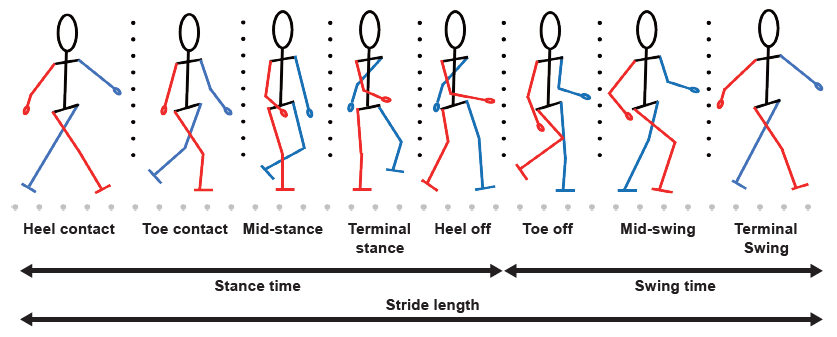
\includegraphics[width=0.7\textwidth]{Images/PhasesOfGaitCycle}
	\caption{Phases of the gait cycle showing the stance and swing phases with key events.} 
		\cite{ZhangWenwen:2022}
		\label{fig:GaitCyclePhase}
	\end{figure}
  Each recorded walking session in the dataset corresponds to the stance and swing phases, as shown in the image, and provides detailed motion data, such as:
 \begin{enumerate}
 	\item	\textbf{Step length:}This is derived from accelerometer data (AX, AY, AZ) and reflects the length of each step in the gait cycle. Parkinsonian gaits often have reduced stride lengths, making this feature critical for classification.
 	
 	\item \textbf{Timing of Gait Phases (Stance and Swing):}The gyroscope data (GX, GY, GZ) helps analyze the timing differences in stance and swing phases. Parkinson’s disease is often associated with prolonged stance phases and shorter, irregular swing phases
 	
 	\item	\textbf{Irregularities in Motion:}Variability in accelerometer and gyroscope readings is a direct indicator of gait anomalies, such as shuffling steps or freezing of gait, which are hallmarks of Parkinsonian gait\cite{WebsterDarter:2019}.
 
 \end{enumerate}
The dataset provides raw sensor data corresponding to these parameters, which align directly with the phases depicted in the gait cycle. By mapping the IMU sensor readings to the gait cycle, the dataset enables precise feature extraction, such as:
\begin{enumerate}
\item Changes in stride length during mid-stance and toe-off.

\item Variability in swing times during mid-swing and terminal swing.

\item Transitions between stance and swing phases.
 \end{enumerate}
This direct correspondence between the dataset and the gait cycle ensures that the model captures the key features needed to differentiate normal and Parkinsonian gaits effectively. By focusing on these parameters, the wearable device provides accurate real-time classification of gait abnormalities\cite{ZhangWenwen:2022}.
\section{Outliers}

Outliers in the dataset refer to data points that deviate significantly from typical walking patterns. Common causes of outliers include:
\begin{enumerate}
\item\textbf{ Sensor misalignment:} Errors caused by improperly placed sensors.

\item \textbf{Abrupt movements:} Sudden stops, turns, or other irregular movements during data collection.

\item \textbf{Participant errors:} Instances where participants failed to follow instructions.
\end{enumerate}
To address outliers, the following steps were taken:
\begin{enumerate}
\item \textbf{Detection:} Statistical methods and visual inspection were used to identify unusual data points.

\item \textbf{Exclusion:} Erroneous data points were removed from the dataset to maintain consistency.

\item \textbf{Correction:} Signal processing techniques, such as filtering, were applied to smooth abrupt spikes in the data\cite{ZhangWenwen:2022}.
\end{enumerate}
Handling outliers ensures that the model focuses on accurate and meaningful patterns rather than being influenced by noise.



\section{Anomalies}

Anomalies refer to unexpected patterns in the data that may not align with typical walking cycles. Examples include:
\begin{enumerate}
\item \textbf{Periods of inactivity:} Instances where participants stood still or stopped walking.

\item\textbf{ Exaggerated movements:} Overemphasized gait patterns during simulation of Parkinsonian gait.

\item \textbf{Sensor drift:} Gradual changes in sensor readings over time.
\end{enumerate}
These anomalies were addressed through:
\begin{enumerate}
\item \textbf{Segmentation:} Only active walking phases were included in the dataset.

\item \textbf{Labeling:} Anomalous data was labeled and excluded from training.

\item \textbf{Normalization:} Data was normalized to reduce variability caused by anomalies\cite{ZhangWenwen:2022}.
\end{enumerate}
By addressing anomalies effectively, the dataset ensures that the machine learning model learns patterns representative of actual gait behaviors.
